%  $Description: Author guidelines and sample document in LaTeX 2.09$
%
%  $Author: ienne $
%  $Date: 1995/09/15 15:20:59 $
%  $Revision: 1.4 $
%
%\documentclass[times, 10pt,twocolumn]{article}
\documentclass[conference,final]{IEEEtran}
\usepackage{latex8}
\usepackage{times}

% Users' option
\usepackage{amssymb}
\usepackage{amsmath}
\usepackage{graphicx}
\usepackage{epstopdf}
\usepackage{color}
\topmargin=0.001in
\usepackage{multirow}
\usepackage{booktabs}
\newif\ifdraft
\drafttrue

\renewcommand{\multirowsetup}{\centering}
\renewcommand{\arraystretch}{1.2}
\def\nyc{\centering}

\ifdraft
\newcommand{\fixme}[1]{ { \bf{ ***FIXME: #1 }} }
\newcommand{\jhanote}[1]{ {\textcolor{red} { ***Jha: #1 }}}
\newcommand{\Nkimnote}[1]{ {\textcolor{green} { ***Nkim: #1 }}}
\newcommand{\skonote}[1]{ {\textcolor{blue} { ***Jeff: #1 }}}
\newcommand{\athotanote}[1]{ {\textcolor{green} { ***athota: #1 }}}
\newcommand{\Jkimnote}[1]{ {\textcolor{red} { ***Jkim: #1 }}}
\newcommand{\yyenote}[1]{ {\textcolor{blue} { ***yye00: #1 }}}
\else
\newcommand{\jhanote}[1]{}
\newcommand{\Nkimnote}[1]{}
\newcommand{\fixme}[1]{}
\newcommand{\skonote}[1]{}
\newcommand{\Jkimnote}[1]{}
\fi
% End of users' option

%\documentstyle[times,art10,twocolumn,latex8]{article}

%-------------------------------------------------------------------------
% take the % away on next line to produce the final camera-ready version
\pagestyle{empty}

\newcommand{\up}{\vspace*{-1em}}
\newcommand{\upp}{\vspace*{-0.5em}}
\newcommand{\ts}{$T_{s}$}


%-------------------------------------------------------------------------
\title{A Hybrid CFD-MD Simulation Framework with Coscheduling and Load Balancing}

\author{
 ~\\[-2em]
 Soon-Heum Ko$^{1}$, Nayong Kim$^{1}$, Abhinav Thota$^{1,2}$ (?), \\
 Dimitris Nikitopoulos$^{3}$, Dorel Moldovan$^{3}$ (?), Shantenu Jha$^{*1,2}$\\
 \small{\emph{$^{1}$Center for Computation \& Technology, Louisiana State University, USA}}\\
 \small{\emph{$^{2}$Department of Computer Science, Louisiana State University, USA}}\\
 \small{\emph{$^{3}$Department of Mechanical Engineering, Louisiana State University, USA}}\\
 \small{\emph{$^{*}$Contact Author}}\\
}

%\thispagestyle{empty}

\begin{document}


\maketitle

\begin{abstract}

\skonote{Title needs change}

 Something
\end{abstract}
\up\up


%-------------------------------------------------------------------------
\section{Introduction and Motivation}

\skonote{\\
- CFD/MD Works: Motivation + Previous Works (Nie, Barakos, Harvard, etc.) \\
- Framework for Multi-physics Applications: Motivation for Co-scheduling of Multiple Applications + Previous Works (including REMD)
 (Maybe we need to refer to co-scheduling of multiple tasks via SGE) \\
- Objectives: Develop a Hybrid CFD/MD Simulation Framework including Domain Science Application Codes and Computational Framework
}


% -------------------------------------------------------------------------
\section{A Hybrid CFD-MD Simulation Approach}

\subsection{Macroscopic Flow Characteristics by Continuum Hypothesis}
\skonote{\\
- Brief Introduction of CFD \\
- Features of a CFD Code: Governing equations and discretization / numerical methods
}

\subsection{Detailed Flow Simulation with Intermolecular Effect}
\skonote{\\
- Brief Introduction of MD \\
- Features of an MD Code: Governing equations with force field/ numerical methods
}

\subsection{Implementation of Hybrid Schemes}
\skonote{\\
- How to Couple: Schematic of layers and their meanings \\
- Coupling Schemes: Governing equations (Constrained MD) and its meaning \\
- Implementation of Coupling Schemes: Which data to exchange, when and how often \\
- How the scheme was implemented on CFD and MD solvers
}

\subsection{Numerical Result of a Nano-scale Couette Flow Simulation}
\skonote{\\
- Solution of Couette Flow\\
a. Discuss the limit of current simulations: unrealistic, algorithmic limitation (like governing equations in CFD), external force in hybrid region\\
b. Compare the result with pure CFD, pure MD and Nie��s work\\
- Parametric Study of (choose one of the following issues for more numerical results)\\
a. Domain Size (CFD/MD/Hybrid) for Solution��s Accuracy and Efficiency\\
b. Layer Size (CFD?MD) and Its Position, Imposing the Velocity via Function\\
c. Sampling (Averaging) Time Scale and Its Interval
}


%-------------------------------------------------------------------------
\section{Construction of a Coupled Multi-physics Simulation Framework with Co-scheduling and Load Balancing}
\subsection{SAGA and SAGA-based Frameworks for Coupled Multi-component Computations}
\skonote{\\
Refer to Section 3 in CCGrid2010
}

%\section{SAGA and SAGA-based Frameworks for Large-Scale and Distributed Computation}

% The Simple API for Grid Applications (SAGA) is an API standardization effort within the Open Grid Forum (OGF)~\cite{ogf_web}, an international standards development body concerned primarily with standards for distributed computing. SAGA provides a simple, POSIX-style API to the most common Grid functions at a sufficiently high-level of abstraction so as to be independent of the diverse and dynamic Grid environments. The SAGA specification defines interfaces for the most common Grid-programming functions grouped as a set of functional packages (Fig.~\ref{Fig:SAGA1}). Some key packages are:


%\begin{figure}
% \begin{center}
%     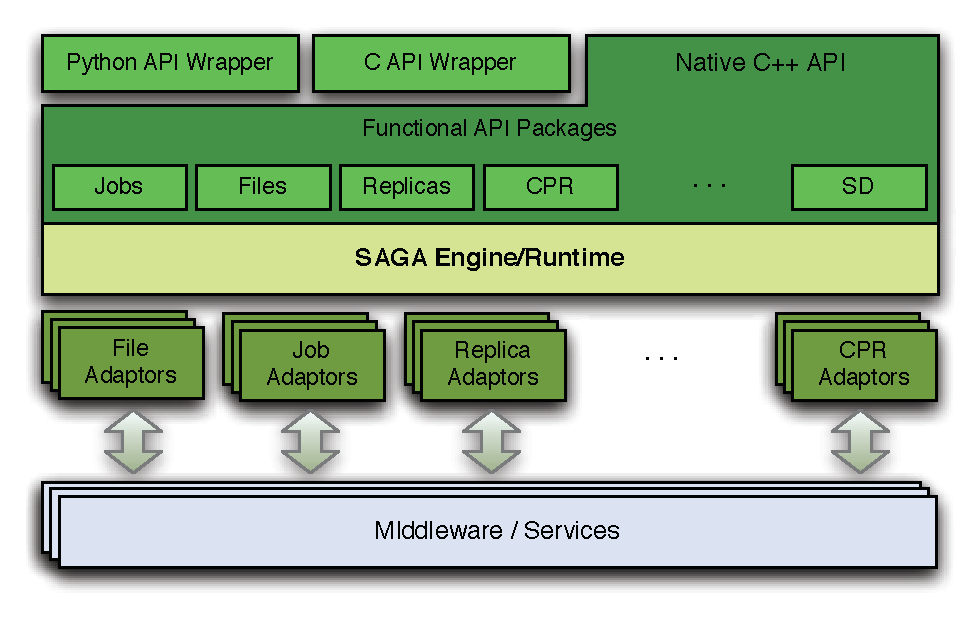
\includegraphics[width=0.40\textwidth]{stci_saga_figures-1.pdf}
% \end{center}
%\caption{\small Layered schematic of the different components of the SAGA landscape. At the topmost level is the simple integrated API which provides the basic functionality for distributed computing. Our BigJob abstraction is built upon this SAGA layer using Python API wrapper}
% \label{Fig:SAGA1}
% \vspace{-1em}
%\end{figure}

%\begin{itemize}
%\item File package - provides methods for accessing local and remote filesystems, browsing directories, moving, copying, and deleting files, setting access permissions, as well as zero-copy reading and writing
%\item Job package - provides methods for describing, submitting, monitoring, and controlling local and remote jobs. Many parts of this package were derived from the largely adopted DRMAA % ~\cite{drmaa_url} specification.
%\item Stream package - provides methods for authenticated local and remote socket connections with hooks to support authorization and encryption schemes.
%\item Other Packages, such as the RPC (remote procedure call) and Replica package
%\end{itemize}


% Fig.~\ref{Fig:BigJob_Structure} shows the structure of BigJob and its operation flow. When a BigJob is submitted to the remote resource, the application manager monitors the status of this pilot-job through the advert service. When resources are allocated to the BigJob, the application manager allots the obtained resources to its sub-jobs and a coupled simulation starts under the control of a multi-physics agent in the remote resource. Advert service keeps on getting the status of a pilot-job from the queuing system and the status of sub-jobs from multi-physics agent and also delivers this information to the application manager by a push-pull mechanism. The application manager watches the status of sub-jobs and decides the next event when the coupled simulation is finished. When one default BigJob is launched, sub-jobs keeps running until final solution is achieved and the manager quits the Pilot-Job at that time. In case multiple BigJobs are submitted for the same simulation or if a load balancing function is included, sub-jobs experience several restarts from their checkpointing data, reflecting changed processor allocation to each application. In the former case, resource allocation to each sub-job follows a pre-defined map according to the number of BigJobs allotted to the simulation; in the latter case, resource allocation to each sub-job becomes dynamic according to its performance, as discussed in the next section.

%%%%% FIGURE %%%%%
%\begin{figure}
%\centering
%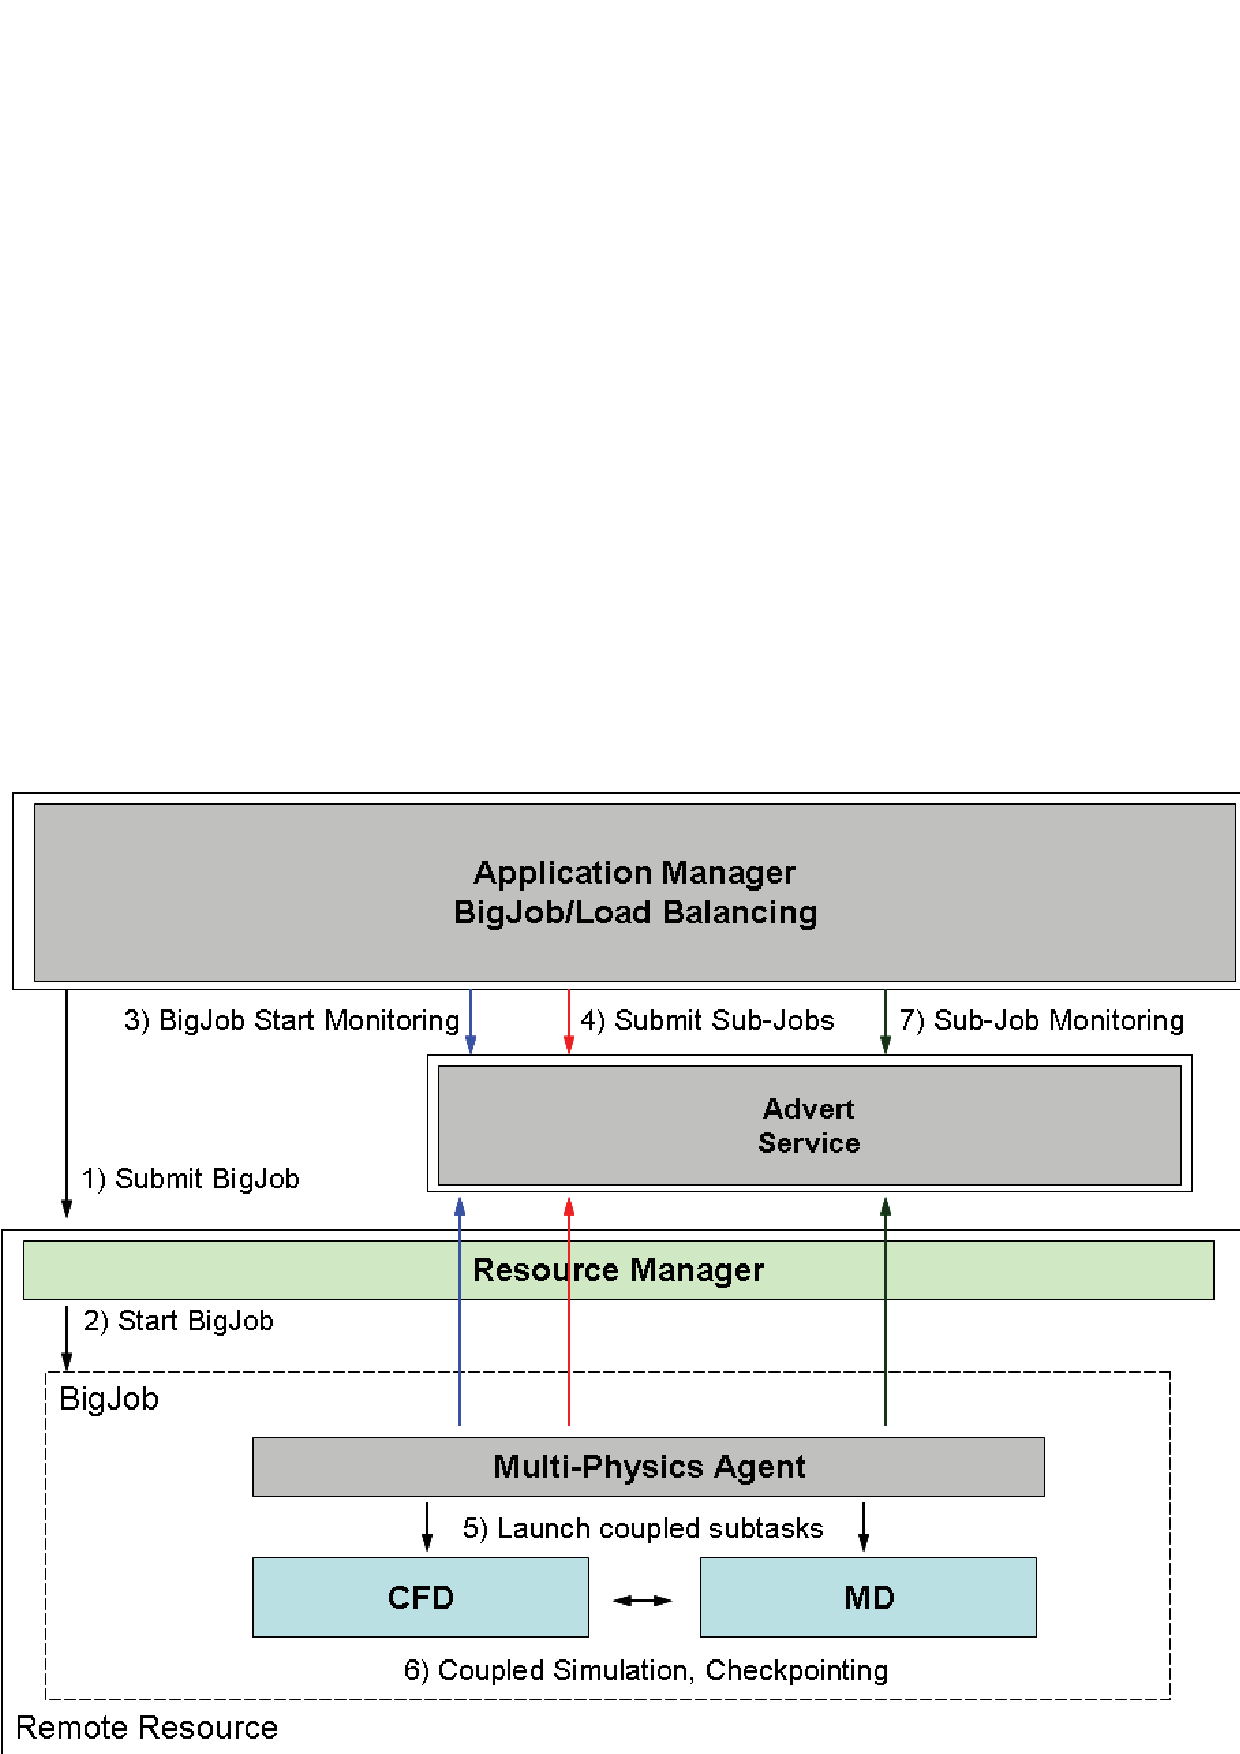
\includegraphics[scale=0.38]{Structure_of_BigJob}
%\caption{\small Architecture of the Controller/Manager and Control Flow: Application manager is responsible for job management including BigJob and sub-job submission, their status monitoring functions. We implement a load balancing module, and migration service based on job information. Application agent system resides on each HPC resource and conducts job information gathering and also communicates with the application manager via the advert service}
%\label{Fig:BigJob_Structure}
%\vspace{-1em}
%\end{figure}
%%%%% FIGURE %%%%%


\subsection{Load Balancing for Coupled Multi-Physics Simulation}
\skonote{\\
- Based on Section 4 in CCGrid 2010: Refine LB, include motivation etc. (e.g., Not touching application codes)
}


%\section{Load Balancing for Coupled Multi-Physics Simulation}

% The flexibility to re-distribute resources (processors) to the individual task does not imply efficient utilization. This is the responsibility of a load-balancer (LB). We will discuss the implementation and algorithm of this LB~\cite{Ko}; it is important to mention that the LB functions in the context of the SAGA-BigJob framework.
% Each application's load is determined by its elapsed time to run the evolution loop. Here, time for initialization or inter-domain data exchange are excluded from the counting, because they are one-time events or irrelevant to application's performance.  The efficient functioning of the LB is predicated on application codes being able to restart from their checkpointing data effectively.  Also, application codes should be equipped with generalized domain partitioning routine to run a simulation with any number of processors, without harming their parallel efficiency a lot. If above conditions are satisfied, it makes sense to load the LB within the pilot-job, to implement dynamic resource allocation between tasks.  Conceptually, the load-balancing algorithm assigns more processors to a sub-task with greater runtime, until the two codes take the same wall-clock time between points when they communicate.
% Interestingly, our approach is very simple and the algorithm is indepenendent of applications upon the predications of,
%(1) each application code follows the ideal parallel efficiency.
%(2) all processors in one node are assigned to one single task.

%Let the computation time (between exchanges) of the two sub-jobs be $t_{CFD}$ and $t_{MD}$, and the number of processors assigned to each domain be $PE_{CFD}$ and $PE_{MD}$, respectively. Subscripts I and F denotes initial and final states. Based on assumption (1), total problem size of each application remains the same after resource re-allocation,

%\vspace{-.2em}
%\footnotesize
%\begin{eqnarray}
%W_{CFD}&=&PE_{CFD,I}\times t_{CFD,I}=PE_{CFD,F}\times t_{CFD,F} \nonumber \\
%W_{MD}&=&PE_{MD,I}\times t_{MD,I}=PE_{MD,F}\times t_{MD,F}
%\label{eq:SimTime_EachTask}
%\end{eqnarray}
%\normalsize

% In spite of the re-allocation, the total number of processors utilized remains the same:

%\vspace{-.2em}
%\footnotesize
%\begin{equation}
%PE_{TOT}=PE_{CFD,I}+PE_{MD,I}=PE_{CFD,F}+PE_{MD,F}
%\label{eq:PECondition}
%\end{equation}
%\normalsize

% Our objective is to reduce the computation time of a sub-job to the point until the two application components show the same computation between the exchange points, i.e., $t_{CFD,F} = t_{MD,F}$. From Equation~\ref{eq:SimTime_EachTask} and Equation~\ref{eq:PECondition} an optimal number of processors distributed for the CFD subtask would be:

%\vspace{-.2em}
%\footnotesize
%\begin{eqnarray}
%PE_{CFD,F} & = & \frac {W_{CFD}} {(W_{CFD} + W_{MD})} \times PE_{TOT}
%\end{eqnarray}
%\normalsize

% The MD simulation (sub-job) will follow a similar expression. The optimal processor distribution from above equation will return a non-integer value. Also, under the second assumption (which is the policy of many supercomputing centers), any load-balancing determined as above, will proceed in discrete values expressed as the multiples of the number of CPU cores in a node. We choose the nearest discrete number to our load balancing as the optimal number of processor on each application.


\subsection{Implementation of an Execution Framework to Support Multi-physics Applications}
\skonote{\\
- Structure of a BigJob\\
- Features of a BigJob Manager (PYTHON)\\
- Changes of Application Codes
}


\subsection{Performance Analysis of a Multi-physics Simulation Framework}
\skonote{\\
- Queue Wait Time Analysis\\
a. Preliminary Test: Waiting Time with Different PX Requests, Wall Time Limit
(Mention that BQP is not perfect, especially measuring inactive waiting time of ��TWO CONVENTIONAL JOBS��)\\
b.Comparison of one BigJob and two conventional jobs at 2-3 locations, with 3 PX settings (128,256,512) and 3 wall time limit (6,24,48)\\
  1) BigJob��s Faster Start by Queuing Policy\\
  2) Co-scheduling and the Safety: Different wall limit time between BigJob and Conventional Jobs due to Highly Unpredictable Inactive Time\\
- Runtime Analysis\\
a. Comparison of LB with conventional simulation time: different system size (with different ratio between CFD and MD), different number of simulation loop and different interval of simulation loop
}


%-------------------------------------------------------------------------
\section{Next Step: Further Refinement}


%-------------------------------------------------------------------------
\section{Conclusions}



\section*{Acknowledgment}
This work is part of the Cybertools (http://cybertools .loni.org)
project and primarily funded by NSF/LEQSF (2007-10)-CyberRII-01.
Important funding for SAGA has been provided by the UK EPSRC grant
number GR/D0766171/1 (via OMII-UK). This work has also been made
possible thanks to computer resources provided by LONI. We thank Andre
Luckow for initial work on BigJob, Lukasz Lacinski for help with SAGA
deployment (via HPCOPS NSF-OCI 0710874) and Joao Abecasis for his work
on the SAGA Condor adaptors.

%-------------------------------------------------------------------------
%\nocite{ex1,ex2}
%\bibliographystyle{IEEEtran}
%\bibliography{saga_tg08}


\end{document}


